\documentclass{article}
\usepackage{enumitem}
\usepackage{tikz}
\usepackage{listings}
\usepackage{graphicx}
\usepackage{xcolor}
\usepackage{amsmath}

\usetikzlibrary{bayesnet}
\lstset{
    basicstyle=\small\ttfamily,
    breaklines=true,
    backgroundcolor=\color{gray!10},
    frame=single,
    numbers=left,
    numberstyle=\tiny,
    captionpos=b,
    language=Python
}

\begin{document}

\title{MATH 4225  \\Foundation of Big Data and Learning\\ Project}
\author{Mustafa Batin EFE\\23501154}
\maketitle
\newpage

\section{Introduction}

In this project, the task is to work with the data obtained from the data.gov.hk. The goal is to develop a PGM and its corresponding generative model.

Firstly, we will load and pre-process the necessary datasets. We will then perform exploratory data analysis and visualization to gain initial insights into the data.

Then, we will conduct a correlation analysis to identify any relationships between the number of taxi accidents and the number of visitors, such as mainland visitors, Hong Kong residents, and tourists. 

After that, we will use MCMC(Markov Chain Monte Carlo) and Gibbs Sampling techniques to perform an analysis and examine the posterior distributions of the parameters. 

Finally, we will use VI (Variational Inference to examine the posterior distributions of the parameters.

\section{Probabilistic Graphical Model}

\begin{itemize}
  \item Used the \texttt{pygraphviz} library to create a Bayesian network graph.
  \item The code renders the graph as a file and displays the image.

  \begin{center}
  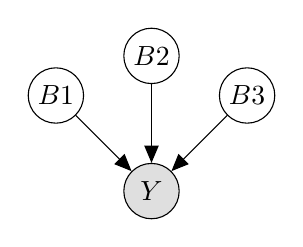
\begin{tikzpicture}

  % Define nodes
  \node[obs] (Y) {$Y$};
  \node[latent, above left=of Y] (B1) {$B1$};
  \node[latent, above=of Y] (B2) {$B2$};
  \node[latent, above right=of Y] (B3) {$B3$};

  % Connect the nodes
  \edge {B1,B2,B3} {Y};

  \end{tikzpicture}
  \end{center}

\end{itemize}



\section{Data Sources and Preprocessing}

\subsection{Data Sources}
The data used for this study was obtained from the following sources:

\subsubsection{Daily Passenger Traffic Data}
\begin{itemize}
  \item Source: Hong Kong Immigration Department
  \item Dataset: Statistics on Daily Passenger Traffic
  \item Resource URL: \url{https://data.gov.hk/en-data/dataset/hk-immd-set5-statistics-daily-passenger-traffic/resource/e06a2a45-fe05-4eb4-9302-237d74343d52}

\end{itemize}

\subsubsection{Accident Data}
\begin{itemize}
  \item Source: Hong Kong Transport Department
  \item Dataset: Monthly Traffic and Transport Digest
  \item Resource URL: \url{https://data.gov.hk/en-data/dataset/hk-td-tis_10-monthly-traffic-and-transport-digest}

\end{itemize}

\subsubsection{Maximum Taxi Involvement Data}
\begin{itemize}
  \item Source: Hong Kong Transport Department
  \item Dataset: Monthly Traffic and Transport Digest (Section 7: Road Traffic Accident Statistics - Table 7.2)
  \item Resource URL: \url{https://data.gov.hk/en-data/dataset/hk-td-tis_10-monthly-traffic-and-transport-digest/resource/3e1c47ab-fed4-4e69-bd22-e2523bca3266}

\end{itemize}

\subsection{Preprocessing}
\subsubsection{Filtering Airport Arrival Data}
The code filters the daily passenger traffic data to include only rows where the control point is "Airport" and the movement is "Arrival." This is done using the following code snippet:

\begin{lstlisting}
airport_arrival_rows = df[(df['Control Point'] == 'Airport') & (df['Arrival / Departure'] == 'Arrival')]
airport_arrival_df = pd.DataFrame(airport_arrival_rows)
\end{lstlisting}

The filtered data is stored in the \texttt{airport\_arrival\_df} DataFrame.

\subsubsection{Converting Date Columns}
The code converts the "Date" column in the \texttt{airport\_arrival\_df} DataFrame to the datetime format using the \texttt{pd.to\_datetime()} function. This is done using the following code snippet:

\begin{lstlisting}
airport_arrival_df['Date'] = pd.to_datetime(airport_arrival_df['Date'], format='%d-%m-%Y')
\end{lstlisting}

\subsubsection{Grouping and Calculating Averages}
The code groups the airport arrival data by month and calculates the average arrivals for each month. This is done separately for Mainland Visitors, Tourist Visitors, and Hong Kong Residents. The code snippet for calculating the average arrivals for tourists is shown below:

\begin{lstlisting}
avg_arrivals_by_month_tourists = airport_arrival_df.groupby('Month')['Tourists'].mean().reset_index()
\end{lstlisting}

Similar code snippets are used to calculate the average arrivals for Mainland Visitors and Hong Kong Residents.

\subsubsection{Filtering Taxi Involvement Data}
The code filters the taxi involvement data to include only rows where the vehicle class code is 3. This is done using the following code snippet:

\begin{lstlisting}
filtered_data = data[data['VEHICLE_CLASS_CODE'] == 3]
filtered_df_taxi = filtered_data[filtered_data['YR_MTH'] > '2021-12-01']
\end{lstlisting}

The filtered data is stored in the \texttt{filtered\_df\_taxi} DataFrame.


\section{Exploratory Data Analysis}
\subsection{Airport Arrivals for Tourists}
\includegraphics[width=\textwidth]{tourists_arrivals.pdf}

\textbf{Description:} This plot represents the average monthly airport arrivals for tourists.

\textbf{Visualization:} The scatter plot and line plot show the trend and variation in average arrivals for tourists each month.

\textbf{Insights:} By analyzing this plot, you can understand the patterns and fluctuations in tourist arrivals over the specified time period (from January 2022 to August 2023).


\subsection{Airport Arrivals for Mainland Visitors}
\includegraphics[width=\textwidth]{mainland_arrivals.pdf}

\textbf{Description:} This plot represents the average monthly airport arrivals for Mainland visitors.

\textbf{Visualization:} Similar to the tourists' plot, it uses scatter and line plots to depict the average arrivals for Mainland visitors each month.

\textbf{Insights:} Examining this plot allows you to gain insights into the trends and variations in arrivals of Mainland visitors over the specified time period.


\subsection{Airport Arrivals for Hong Kong Residents}
\includegraphics[width=\textwidth]{residents_arrivals.pdf}

\textbf{Description:} This plot represents the average monthly airport arrivals for Hong Kong residents.

\textbf{Visualization:} It utilizes scatter and line plots to illustrate the average arrivals for Hong Kong residents on a monthly basis.

\textbf{Insights:} Analyzing this plot helps in understanding how the airport arrivals for Hong Kong residents have been changing over the specified time period.


\subsection{Number of Taxi Involved in Accidents}
\includegraphics[width=\textwidth]{taxi_involvement.pdf}

\textbf{Description:}This plot represents the number of taxi-involved accidents over time.

\textbf{Visualization:}It utilizes both scatter and line plots with red dots to illustrate the monthly variation in the number of taxi-involved accidents.

\textbf{Insights:}Analyzing this plot helps in understanding how the frequency of taxi-involved accidents has been changing over the specified time period, with a focus on months after December 2021.


\section{Correlation Analysis}
\includegraphics[width=\textwidth]{heatmap.pdf}
\subsection*{Taxi Number Involved in Accident vs. Mainland Visitors (0.588797):}

There is a moderate positive correlation ($0.588797$) between the number of taxi accidents (`Taxi Number') and the number of Mainland Visitors. This suggests that as the number of Mainland Visitors increases, the number of taxi accidents tends to increase, but the correlation is not extremely strong.

\subsection*{Taxi Number Involved in Accident vs. Hong Kong Residents (0.536850):}

There is a moderate positive correlation ($0.536850$) between the number of taxi accidents and the number of Hong Kong Residents. This implies that there is a tendency for an increase in taxi accidents as the number of Hong Kong Residents increases.

\subsection*{Taxi Number Involved in Accident vs. Tourists (0.533777):}

There is a moderate positive correlation ($0.533777$) between the number of taxi accidents and the number of Tourists. This suggests a similar pattern as observed with Mainland Visitors and Hong Kong Residents.

\subsection*{Mainland Visitors vs. Hong Kong Residents (0.952173):}

There is a very strong positive correlation ($0.952173$) between the number of Mainland Visitors and Hong Kong Residents. This indicates a close relationship where an increase in Mainland Visitors is highly correlated with an increase in Hong Kong Residents.

\subsection*{Mainland Visitors vs. Tourists (0.980271):}

There is a very strong positive correlation ($0.980271$) between the number of Mainland Visitors and Tourists. This implies a close relationship where an increase in Mainland Visitors is highly correlated with an increase in Tourists.

\subsection*{Hong Kong Residents vs. Tourists (0.945693):}

There is a very strong positive correlation ($0.945693$) between the number of Hong Kong Residents and Tourists. This indicates a close relationship where an increase in Hong Kong Residents is highly correlated with an increase in Tourists.

Overall, the correlation matrix provides insights into the relationships between taxi accidents and the number of visitors from different backgrounds. The strong correlations among the visitor categories suggest a potential common factor influencing their numbers. 
\newpage
\section{MCMC and Gibbs Sampling}

For simplicity, let's denote:

\begin{align*}
y & : \text{Response variable (e.g., accidents)} \\
X_1 & : \text{Predictor variable 1 (e.g., mainland\_visitors)} \\
X_2 & : \text{Predictor variable 2 (e.g., tourists)} \\
X_3 & : \text{Predictor variable 3 (e.g., locals)} \\
B_1 & : \text{Coefficient for } X_1 \\
B_2 & : \text{Coefficient for } X_2 \\
B_3 & : \text{Coefficient for } X_3 \\
\sigma_{\text{sq}} & : \text{Variance}
\end{align*}

The likelihood function for a linear regression model is assumed to follow a normal distribution:

\[
P(y | B_1, B_2, B_3, \sigma_{\text{sq}}) = \frac{1}{\sqrt{2\pi\sigma_{\text{sq}}}} \exp\left(-\frac{(y - (B_1X_1 + B_2X_2 + B_3X_3))^2}{2\sigma_{\text{sq}}}\right)
\]

The prior distributions for the coefficients are assumed to be normal distributions:

\[
P(B_1) = \frac{1}{\sqrt{2\pi\sigma_{B_1}^2}} \exp\left(-\frac{B_1^2}{2\sigma_{B_1}^2}\right)
\]
\[
P(B_2) = \frac{1}{\sqrt{2\pi\sigma_{B_2}^2}} \exp\left(-\frac{B_2^2}{2\sigma_{B_2}^2}\right)
\]
\[
P(B_3) = \frac{1}{\sqrt{2\pi\sigma_{B_3}^2}} \exp\left(-\frac{B_3^2}{2\sigma_{B_3}^2}\right)
\]

The posterior distributions for the coefficients are then proportional to the product of the likelihood and the priors:

\[
P(B_1 | y, X_1, X_2, X_3) \propto P(y | B_1, B_2, B_3, \sigma_{\text{sq}}) \times P(B_1)
\]
\[
P(B_2 | y, X_1, X_2, X_3) \propto P(y | B_1, B_2, B_3, \sigma_{\text{sq}}) \times P(B_2)
\]
\[
P(B_3 | y, X_1, X_2, X_3) \propto P(y | B_1, B_2, B_3, \sigma_{\text{sq}}) \times P(B_3)
\]

Then, we use Metropolis-Hastings algorithm to sample. 

Note: Normal distribution is used as the proposal distribution for each parameter.
\newpage
\begin{enumerate}[label=\arabic*.]
    \item \textbf{Initialization of Parameters:}
    \begin{lstlisting}
    B1 = 0  # Mainland Visitors
    B2 = 0  # Tourists
    B3 = 0  # Residents
    \end{lstlisting}
    
    The parameters \(B1\), \(B2\), and \(B3\) are initialized to zero. These parameters represent coefficients associated with Mainland Visitors, Tourists, and Residents, respectively.

    \item \textbf{Setting Up Iterations and Data:}
    \begin{lstlisting}
    N_iter = 1000
    samples = np.zeros((N_iter, 3))
    accidents = filtered_df_taxi['NO_VEHICLE']
    mainland_visitors = avg_arrivals_by_month_mainland['Mainland Visitors']
    tourists = avg_arrivals_by_month_tourists['Tourists']
    locals = avg_arrivals_by_month_residents['Hong Kong Residents']
    N = len(accidents)
    \end{lstlisting}
    
    The number of iterations (\(N_{\text{iter}}\)) is set to 1000, and placeholders are created to store samples. Relevant data such as accidents, mainland visitors, tourists, and locals are loaded from dataframes.

    \item \textbf{Markov Chain Monte Carlo (MCMC) Sampling:}
    \begin{lstlisting}
    for i in range(N_iter):
        # Sampling B1
        # ... (update B1 based on sampled values)

        # Sampling B2
        # ... (update B2 based on sampled values)

        # Sampling B3
        # ... (update B3 based on sampled values)

        samples[i, :] = [B1, B2, B3]
    \end{lstlisting}

    The MCMC loop iteratively updates parameters (\(B1\), \(B2\), \(B3\)) based on sampled values using normal distribution. The update formulas involve calculations related to data.

    \item \textbf{Burn-In Period and Posterior Distributions:}
    \begin{lstlisting}
    burn_in = int(N_iter * 0.1)
    posterior_B1 = samples[burn_in:, 0]
    posterior_B2 = samples[burn_in:, 1]
    posterior_B3 = samples[burn_in:, 2]
    \end{lstlisting}

    A burn-in period is defined (discarding initial samples), and posterior distributions of parameters (\(B1\), \(B2\), \(B3\)) are extracted from MCMC samples.

\end{enumerate}


\subsection{Results}

\subsubsection*{Parameter: \(B1\) Posterior}
\begin{itemize}
    \item Effect on Accidents (1.0 Positive to 0.0 $\rightarrow$ Negative) = 0.45222222222222225
    \item Mean: -1.654735237092731e-05
    \item Median: -5.1664493283096606e-05
    \item Standard deviation: 0.0004238580034395113
    \item Interquartile range: 0.0006459896115224824
\end{itemize}

\subsubsection*{Parameter: \(B2\) Posterior}
\begin{itemize}
    \item Effect on Accidents (1.0 Positive to 0.0 $\rightarrow$ Negative) = 0.5044444444444445
    \item Mean: 5.62337158564161e-06
    \item Median: 6.334585317296868e-06
    \item Standard deviation: 0.00026982959376700607
    \item Interquartile range: 0.0003754271059697741
\end{itemize}

\subsubsection*{Parameter: \(B3\) Posterior}
\begin{itemize}
    \item Effect on Accidents (1.0 Positive to 0.0 $\rightarrow$ Negative) = 0.5766666666666667
    \item Mean: 2.7350132733917572e-06
    \item Median: 1.1096929669754101e-05
    \item Standard deviation: 6.405233217248062e-05
    \item Interquartile range: 6.901099954962191e-05
\end{itemize}

\subsubsection*{Parameter: \(B1\)}
\begin{itemize}
    \item HPDI: [-0.00072511, 0.00076627]
    \item \(B1\) lies within the 95\% HPDI.
\end{itemize}

\subsubsection*{Parameter: \(B2\)}
\begin{itemize}
    \item HPDI: [-0.00045037, 0.00051407]
    \item \(B2\) lies within the 95\% HPDI.
\end{itemize}

\subsubsection*{Parameter: \(B3\)}
\begin{itemize}
    \item HPDI: [-0.00011837, 0.00013067]
    \item \(B3\) lies within the 95\% HPDI.
\end{itemize}

\subsection{Outcome}

\subsubsection{Parameter: B1 Posterior}
\begin{itemize}
    \item Effect on Accidents (1.0 Positive to 0.0 $\rightarrow$ Negative): $0.452$
    \item Mean: $-1.6547 \times 10^{-5}$
    \item Median: $-5.1664 \times 10^{-5}$
    \item Standard deviation: $0.0004239$
    \item Interquartile range: $0.000646$
\end{itemize}

\subsubsection{Parameter: B2 Posterior}
\begin{itemize}
    \item Effect on Accidents (1.0 Positive to 0.0 $\rightarrow$ Negative): $0.504$
    \item Mean: $5.6234 \times 10^{-6}$
    \item Median: $6.3346 \times 10^{-6}$
    \item Standard deviation: $0.0002698$
    \item Interquartile range: $0.0003754$
\end{itemize}

\subsubsection{Parameter: B3 Posterior}
\begin{itemize}
    \item Effect on Accidents (1.0 Positive to 0.0 $\rightarrow$ Negative): $0.577$
    \item Mean: $2.7350 \times 10^{-6}$
    \item Median: $1.1097 \times 10^{-5}$
    \item Standard deviation: $6.4052 \times 10^{-5}$
    \item Interquartile range: $6.9011 \times 10^{-5}$
\end{itemize}

\subsubsection{Parameter: B1}
\begin{itemize}
    \item HPDI: $[-0.00072511, 0.00076627]$
    \item B1 lies within the 95\% HPDI.
\end{itemize}

\subsubsection{Parameter: B2}
\begin{itemize}
    \item HPDI: $[-0.00045037, 0.00051407]$
    \item B2 lies within the 95\% HPDI.
\end{itemize}

\subsubsection{Parameter: B3}
\begin{itemize}
    \item HPDI: $[-0.00011837, 0.00013067]$
    \item B3 lies within the 95\% HPDI.
\end{itemize}


    


\section{MCMC and VI}
\subsubsection*{Likelihood Function:}

\[
P(\mathbf{y} \mid B_1, B_2, B_3, \sigma_{\text{sq}}) = \prod_{i=1}^{N} \frac{1}{\sqrt{2\pi\sigma_{\text{sq}}^2}} \exp\left(-\frac{(y_i - \hat{y}_i)^2}{2\sigma_{\text{sq}}^2}\right)
\]
where:
\begin{align*}
&\mathbf{y} \text{ is the vector of observed response variables,} \\
&\hat{y}_i \text{ is the predicted value for the }i\text{-th observation,} \\
&\sigma_{\text{sq}} \text{ is the standard deviation of the likelihood.}
\end{align*}

\subsubsection*{Prior Distributions:}
Note: \(B_1\), \(B_2\), and \(B_3\) are assumed to be normal distributions.

\[
P(B_1) = \frac{1}{\sqrt{2\pi\sigma_{B_1}^2}} \exp\left(-\frac{B_1^2}{2\sigma_{B_1}^2}\right)
\]
\[
P(B_2) = \frac{1}{\sqrt{2\pi\sigma_{B_2}^2}} \exp\left(-\frac{B_2^2}{2\sigma_{B_2}^2}\right)
\]
\[
P(B_3) = \frac{1}{\sqrt{2\pi\sigma_{B_3}^2}} \exp\left(-\frac{B_3^2}{2\sigma_{B_3}^2}\right)
\]
where:
\begin{align*}
&\sigma_{B_1}^2, \sigma_{B_2}^2, \text{ and } \sigma_{B_3}^2 \text{ are the variances of the priors for }B_1, B_2, \text{ and } B_3 \text{ respectively.}
\end{align*}

\subsubsection*{Posterior Distributions:}

\[
P(B_1 \mid \mathbf{y}, X_1, X_2, X_3) \propto P(\mathbf{y} \mid B_1, B_2, B_3, \sigma_{\text{sq}}) \times P(B_1)
\]
\[
P(B_2 \mid \mathbf{y}, X_1, X_2, X_3) \propto P(\mathbf{y} \mid B_1, B_2, B_3, \sigma_{\text{sq}}) \times P(B_2)
\]
\[
P(B_3 \mid \mathbf{y}, X_1, X_2, X_3) \propto P(\mathbf{y} \mid B_1, B_2, B_3, \sigma_{\text{sq}}) \times P(B_3)
\]

\subsubsection*{Optimization:}
The code uses the Adam optimizer to minimize the negative log joint probability, which is equivalent to maximizing the log joint probability.

\subsubsection*{Variational Inference:}
The final step involves using variational inference to obtain samples from the posterior distribution.


\begin{enumerate}
    \item \textbf{Data Loading:}
\begin{lstlisting}[language=Python, caption={Data Loading}, label={lst:data_loading}]
accidents = filtered_df_taxi['NO_VEHICLE']
mainland_visitors = avg_arrivals_by_month_mainland['Mainland Visitors']
tourists = avg_arrivals_by_month_tourists['Tourists']
locals = avg_arrivals_by_month_residents['Hong Kong Residents']
\end{lstlisting}
This part loads the necessary data: \texttt{accidents}, \texttt{mainland\_visitors}, \texttt{tourists}, and \texttt{locals} from specific columns of DataFrames (\texttt{filtered\_df\_taxi}, \texttt{avg\_arrivals\_by\_month\_mainland}, \texttt{avg\_arrivals\_by\_month\_tourists}, \texttt{avg\_arrivals\_by\_month\_residents}).

    \item \textbf{TensorFlow Probability Setup:}
\begin{lstlisting}[language=Python, caption={TensorFlow Probability Setup}, label={lst:tfp_setup}]
tfd = tfp.distributions
\end{lstlisting}
This line creates a shorthand reference (\texttt{tfd}) for the \texttt{tensorflow\_probability.distributions} module.

    \item \textbf{Variable Initialization:}
\begin{lstlisting}[language=Python, caption={Variable Initialization}, label={lst:variable_init}]
B1 = tf.Variable(0.0, dtype=tf.float32)
B2 = tf.Variable(0.0, dtype=tf.float32)
B3 = tf.Variable(0.0, dtype=tf.float32)
\end{lstlisting}
Three TensorFlow variables (\texttt{B1}, \texttt{B2}, and \texttt{B3}) are initialized as trainable parameters with an initial value of \texttt{0.0} and data type \texttt{tf.float32}.

    \item \textbf{Log Joint Probability Function:}
\begin{lstlisting}[language=Python, caption={Log Joint Probability Function}, label={lst:log_joint_prob}]
def log_joint_prob(B1, B2, B3):
    # ... (Normalization of data)
    # ... (Model using normalized data)
    # ... (Calculation of log likelihood)
    # ... (Priors for B1, B2, B3)
    return (prior_B1.log_prob(B1) + prior_B2.log_prob(B2) + prior_B3.log_prob(B3) + log_likelihood)
\end{lstlisting}
This function calculates the log joint probability of the Bayesian model, including the log likelihood and prior terms for the parameters \texttt{B1}, \texttt{B2}, and \texttt{B3}.

    \item \textbf{Loss Function:}
\begin{lstlisting}[language=Python, caption={Loss Function}, label={lst:loss_function}]
@tf.function
def loss():
    return -log_joint_prob(B1, B2, B3)
\end{lstlisting}
The loss function is defined as the negation of the log joint probability. The \texttt{@tf.function} decorator is used to convert the function into a TensorFlow graph for optimization.

    \item \textbf{Optimizer Setup:}
\begin{lstlisting}[language=Python, caption={Optimizer Setup}, label={lst:optimizer_setup}]
optimizer = tf.keras.optimizers.Adam(learning_rate=0.01)
\end{lstlisting}
An Adam optimizer with a learning rate of \texttt{0.01} is initialized.

    \item \textbf{Training Loop:}
\begin{lstlisting}[language=Python, caption={Training Loop}, label={lst:training_loop}]
N_iter = 1000
for i in range(N_iter):
    # ... (Gradient Tape to compute gradients)
    # ... (Optimizer applies gradients to update parameters)
\end{lstlisting}
A training loop runs for \texttt{N\_iter} iterations. Inside the loop, a gradient tape is used to compute gradients of the loss with respect to the parameters, and the optimizer applies these gradients to update the parameters.

    \item \textbf{Posterior Distribution Sampling:}
\begin{lstlisting}[language=Python, caption={Posterior Distribution Sampling}, label={lst:posterior_sampling}]
variational_distribution = tfd.MultivariateNormalDiag(loc=[B1, B2, B3], scale_diag=[1.0, 1.0, 1.0])
posterior_samples = variational_distribution.sample(N_iter)
\end{lstlisting}
A multivariate normal distribution is defined based on the learned parameters, and samples from this distribution are drawn. These samples represent the posterior distribution of the parameters.
\end{enumerate}

\subsection{Results}
\includegraphics[width=\textwidth]{snsPosteriors.pdf}
\includegraphics[width=\textwidth]{snsSingle_1.pdf}
\includegraphics[width=\textwidth]{snsSingle_2.pdf}
\includegraphics[width=\textwidth]{snsSingle_3.pdf}

\subsection{Outcome}

\textbf{Mean:}

The mean values represent the central tendency of your posterior distribution for each parameter.

\[
\begin{align*}
B1 & : 0.06775 \\
B2 & : -0.03778 \\
B3 & : 0.01665 \\
\end{align*}
\]

\textbf{Standard Deviation:}

The standard deviation provides a measure of the spread or uncertainty in your parameter estimates.

\[
\begin{align*}
B1 & : 0.97111 \\
B2 & : 0.99863 \\
B3 & : 0.97493 \\
\end{align*}
\]

\textbf{95\% Credible Interval:}

The 95\% credible interval indicates the range in which you are 95\% confident that the true parameter value lies.

\[
\begin{align*}
\text{For } B1 & : [-1.85397, 1.98181] \\
\text{For } B2 & : [-1.97905, 2.08504] \\
\text{For } B3 & : [-1.86814, 1.93454] \\
\end{align*}
\]

\textbf{Interpretation:}

It seems that the mean values are close to zero for each parameter. It shows that the predictors may not have a strong impact on the response variable. However, the wide credible intervals indicate significant uncertainty in these estimates.

\end{document}
